\documentclass[handout]{beamer}

\input{../Vor2017glærur}

\title{Tölvunarfræði 2}
\subtitle{Vika 1}

\begin{document}

\begin{frame}
\titlepage
\end{frame}

\section{Um námskeiðið}

\begin{frame}{Kennari}
Upplýsingaskjal um námskeiðið má finna á Uglu!
\end{frame}

\section{C++}

\begin{frame}{C++}
\begin{itemize}
 \item C++ er almennt forritunarmál, notað á ýmsum sviðum
 \item Yfirleitt litið á það sem ``mid-level'' forritunarmál í dag
 \begin{itemize}
  \item Höfum ýmis þægindi sem við búumst við af nútímaforritunarmálum
  \item Höfum líka ýmsa möguleika á beinni minnisstjórnun
 \end{itemize}
 \item Kom út snemma á 9. áratugnum, hefur verið mjög áhrifamikið
\end{itemize}
\end{frame}

\begin{frame}[fragile]{Hello World forrit í C++}
Hið hefðbundna forrit sem skrifar út ``halló heimur'', í C++:
\cppfile[label=hello.cpp]{Code/w1/hello.cpp}
Þessa skrá mætti búa til í hvaða textaritli (e. \emph{plaintext editor}) sem er.
\end{frame}

\begin{frame}[fragile]{Hvað erum við að horfa á?}
\begin{itemize}
 \item \texttt{\#include <iostream>}: Veitir okkur aðgang að staðalstraumum
 \item \texttt{int main()}: Skilgreining falls að nafni \texttt{main} sem tekur engin inntök og skilar heiltölu
 \begin{itemize}
  \item Afmarkað með slaufusvigum
 \end{itemize}
 \item \verb|std::cout << "Halló heimur!" << std::endl;|: Strengurinn ``halló heimur'' skrifaður á ``console out'' strauminn með straumsinnsetningarvirkjanum \verb|<<| ásamt boðum um að línunni sé lokið
 \item \texttt{return 0;}: Heiltölunni 0 skilað, sem þýðir að fallið hafi lokið keyrslu rétt
\end{itemize}
\end{frame}

\begin{frame}[fragile]{Þýðing C++ forrits}
C++ kóði er undantekningalítið þýddur. Dæmi um þýðanda er \href{https://gcc.gnu.org/}{GCC}, sem kalla má á af skipanalínu:
\begin{minted}[frame=lines]{bash}
$ g++ hello.cpp -o hello
$ ./hello
Halló heimur!
\end{minted}
Hér er \texttt{g++} skipunin sem keyrir upp GCC þýðandann fyrir forritskóðaskrána \texttt{hello.cpp} og býr til keyranlegu skrána \texttt{hello}.
\end{frame}

\begin{frame}{Undir húddinu}
\begin{columns}
\column{0.66\textwidth}
Það að mynda keyrsluskrá út frá C++ kóða fer fram í nokkrum (hér einfölduðum) skrefum.
\begin{enumerate}
 \item Forritskóðinn fer í gegnum forþýðanda (e. \emph{preprocessor}), sem sækir \texttt{\#include}-aðan kóða, framkvæmir textaútskiptingar o.fl.
 \item Útvíkkaði kóðinn er þýddur (e. \emph{compiled})
 \item Þýddi kóðinn er tengdur (e. \emph{linked}) svo úr verði keyranleg skrá
\end{enumerate}
\column{0.33\textwidth}
\begin{center}
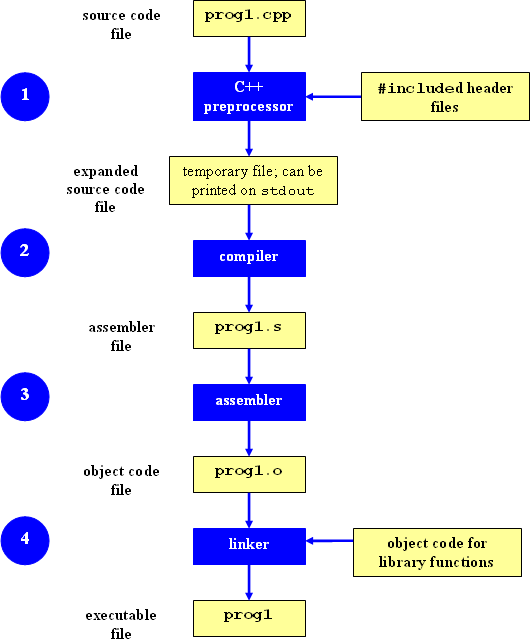
\includegraphics[width=1.1\linewidth]{compile}

{\tiny \href{http://faculty.cs.niu.edu/~mcmahon/CS241/Notes/compile.html}{Útskýring/uppruni myndar} }
\end{center}
\end{columns}
\end{frame}

\begin{frame}[fragile]{Hvar er þessi þýðandi keyrður?}
\begin{itemize}
 \item Við munum kynnast skipanalínunni
 \begin{itemize}
  \item Á Windows: keyra cmd.exe
  \item Á Mökkum: finna terminal
  \item Á Linux: Ýmis nöfn, en á að vera auðfinnanlegt
 \end{itemize}
 \item Hægt er að athuga hvort að GCC sé uppsett með því að keyra
\end{itemize}
\begin{minted}[frame=lines]{bash}
$ g++ --version
g++ (Ubuntu 5.4.0-6ubuntu1~16.04.4) 5.4.0 20160609
\end{minted}

\end{frame}


\begin{frame}{Uppsetning GCC}
\begin{itemize}
 \item Windows (bein uppsetning):
 \begin{itemize}
  \item Setja upp MinGW eða MinGW-w64
  \item Síðan þarf að passa að GCC sé í PATH
 \end{itemize}
 \item Windows (cygwin)
 \begin{itemize}
  \item Setja upp Cygwin með \texttt{gcc-core} og \texttt{gcc-g++} pökkunum
 \end{itemize}
 \item Makkar: 
 \begin{itemize}
  \item Setja upp homebrew og ``xcode command line tools''
 \end{itemize}
 \item Linux:
 \begin{itemize}
  \item Það er í pakkakerfinu ef ekki foruppsett
  \item \texttt{sudo apt-get install build-essential} á Ubuntu
 \end{itemize}
 \item Hægt er að komast fram hjá uppsetningu með því að nota (gamla) útgáfu af GCC á \texttt{hekla.rhi.hi.is} í gegnum ssh
\end{itemize}
\end{frame}



\begin{frame}{Næst}
\end{frame}


\end{document}
